\documentclass{article}
\usepackage{graphicx} % Required for inserting images
\usepackage{float}
\usepackage{subcaption}
\usepackage{amsmath}
\begin{document}

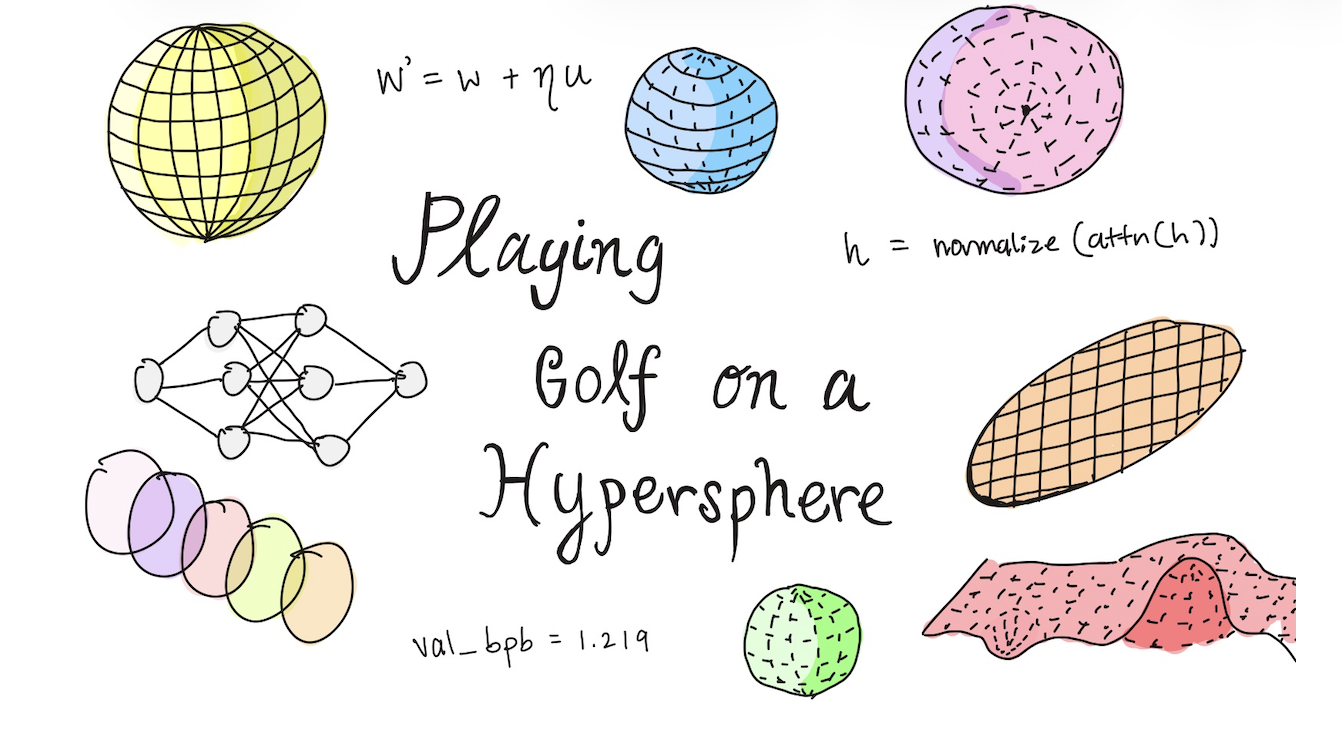
\includegraphics[width=\linewidth]{hypersphere.png}

About four weeks ago, I stumbled across the OpenAI Parameter Golf Challenge. Inspired by the nanoGPT speedrun, Parameter Golf challenges participants to optimize val bpb loss under a submission size constraint of 16mb. Feeling adventurous, I opted to try and patch together a creative submission, ultimately leading me to experiment with manifold constrained architectures. Specifically, I spent the majority of the challenge playing around with the nGPT architecture and trying to adapt the Muon optimizer to the hypersphere geometry. Current Riemannian optimizers are either computationally expensive, or are specifically designed for fixed low rank matrices (LoRA). Since Muon does not naturally produce gradients that are tangent to the hypersphere, a significant portion (approximately 12\%)of the update signal is wasted in the non-tangential direction. 

This work was conducted alongside Max Lovitt. Thank you to OpenAI for sponsoring \$525 worth of compute credits via Runpod which made all of these experiments possible.

\section{Introduction}
This blog will focus less on techniques which optimized for the Parameter Golf and rather on my investigation on the nGPT. All of the work, however, was motivated by the guidelines of the challenge. In order to maximize parameter efficiency of a model, it is natural to try and maximize the expressiveness of the model, which is a proposed benefit of manifold constrained architectures. The nGPT, proposed by Loshchilov et al., projects the representations and weights at every intermediate step of a transformer onto a hypersphere. Residual accumulation uses an approximation of SLERP (Spherical Linear Interpolation) to model learning representations as learning a point on the surface of this hypersphere. Due to the strong normalization built into the architecture, no LayerNorm or RMSNorm layers are used. MLP layers are implemented as SwigLU MLPs. The original paper uses the Adam optimizer, and since Muon has been the go-to optimizer in SOTA language models, our goal is to measure and try to adapt the Muon optimizer to this architecture.

In this blog post, we will discuss the following:
\begin{itemize}
\item a negative result indicating information in the radial component of gradient updates is mostly negligible to training when using a naive update projection on the manifold
\item Newton-Schulz reinjecting radial alignment in the gradient updates for our weights

\end{itemize}

\section{The Radial Component}

We begin with some math. Consider an nGPT model $N$, and let $w$ be the a vector in its weight matrices that lies on the hypersphere that the parameters of $N$ is constrained to. Suppose the gradient update produced by Muon, post Newton-Schulz and momentum, is $u$. It is important to note that $\lVert \mathbf{w} \rVert =1, \lVert \mathbf{u} \rVert = 1.$ Then, for some sufficiently small step size $\eta$, we have that the updated weight $ \mathbf{w}' $ is:
$$ \mathbf{w}'  = \mathbf{w} + \eta \mathbf{u}.$$
However, since $N$ projects all of its parameters back onto the hypersphere after each update, we have that:
$$ \mathbf{w}' _{\text{final}}=\frac{ \mathbf{w}' }{\lVert  \mathbf{w}' \rVert}.$$
Intuitively, this means that for sufficiently small $\eta,$ the meaningful part of the update is the one which is tangential to the surface of the hypersphere since the radially aligned component is squashed by magnitude normalization. Define $$\mathbf{u}'=\langle \mathbf{u},\mathbf{w} \rangle \mathbf{w}$$ and $\mathbf{u}^\perp = \mathbf{u}-\langle \mathbf{u},\mathbf{w} \rangle \mathbf{w}$. Then we have:

\begin{align*}
 \mathbf{w}'  
& = \mathbf{w} + \eta (\mathbf{u}' + \mathbf{u}^\perp) \\
& = \mathbf{w} + \eta(\langle \mathbf{u},\mathbf{w} \rangle \mathbf{w} + \mathbf{u}^\perp) \\
& = \mathbf{w} + \eta \langle \mathbf{u},\mathbf{w} \rangle \mathbf{w} + \eta \mathbf{u}^\perp \\
& = \mathbf{w} (1 +\eta \langle \mathbf{u},\mathbf{w} \rangle) + \eta \mathbf{u}^\perp.
\end{align*} 


Building off our assumption that $\eta$ is sufficiently small enough, we have that:

\begin{align*}
\lVert \mathbf{w'} \rVert ^2
& = \lVert \mathbf{w} \rVert^2(1 + 2\eta \langle \mathbf{u},\mathbf{w} \rangle + \eta^2 \langle \mathbf{u}, \mathbf{w} \rangle^2) + \eta^2 \lVert \mathbf{u}^\perp \rVert^2 \\
& = 1 + 2\eta \langle \mathbf{u},\mathbf{w} \rangle + \eta^2 \langle \mathbf{u}, \mathbf{w} \rangle^2 + \eta^2 \lVert \mathbf{u}^\perp \rVert^2 \\
& \approx 1 + 2\eta \langle \mathbf{u},\mathbf{w} \rangle + \eta^2 \langle \mathbf{u}, \mathbf{w} \rangle^2 \\
& = (1 + \eta\langle \mathbf{u}, \mathbf{w} \rangle)^2
\end{align*}

giving $\lVert \mathbf{w}' \rVert \approx 1 + \eta \langle \mathbf{u},\mathbf{w} \rangle$. Hence,

$$\mathbf{w}'_\text{final} = \frac{\mathbf{w} (1 +\eta \langle \mathbf{u},\mathbf{w} \rangle) + \eta \mathbf{u}^\perp}{1 + \eta \langle \mathbf{u},\mathbf{w} \rangle}=\mathbf{w} + \frac{\eta \mathbf{u}^\perp}{1+\eta \langle \mathbf{u}, \mathbf{w} \rangle}.$$

Interestingly, the radial component $u'$ is completely removed from the equation (of course, under the assumption that $\eta$ is sufficiently small). 
\\
\\
What does this mean for our update gradient $\mathbf{u}$? Well, if the relative magnitude of the radial component $\mathbf{u}'$ is large, a significant portion of our signal is lost to normalization. From this, there are a number of natural directions that we can explore.

\section{Set up}

Experiments were conducted on two, slightly different, nGPT models. Both models followed the standard implementation of the nGPT, as referenced in Loshchilov et al. Transformer blocks were implemented with RoPE, multi-headed attention, and SwigLU MLPs. \newline

Our training setup for the two models differed only by a single computation pre-Newton-Schulz. The baseline model computes gradients just like the standard Muon optimizer, and our modified model projects the gradient matrix onto the hypersphere prior to Newton-Schulz. \newline

Why project into the tangent space prior to Newton-Schulz if this does not guarantee the transformed gradient to also be tangentially aligned? Two reasons.

The main benefit of the Muon optimizer is in the balancing of the singular values. If the Newton Schulz step is operating on a matrix with radially aligned information, it is possible that Newton Schulz is wasting signal by balancing the singular values along a radially aligned axis. We hypothesize that pre-projection may correct for this loss.

Models were trained with the following set up:
\begin{itemize}
    \item num\_layers=9
    \item d\_model=512
    \item num\_heads=8
    \item alpha\_s\_init=0.05
    \item qk\_s\_init=1.0
    \item qk\_s\_scale=1.0
    \item mlp\_s\_init=1.0
    \item mlp\_s\_scale=1.0
    \item train\_batch=524\_288
    \item val\_batch=524\_288
    \item num\_steps=9810 (number of steps the baseline could fit in 10 minutes)
\end{itemize}

\section{Findings}

We present findings suggesting that for the naive implementation of a hypersphere adapted Muon, discarding the radial component does not yield measurable benefit. Furthermore, we hypothesize that pre-projecting the update gradient onto the tangent space fails to even get rid of the final update's radial alignment.

The first notable find was that the naive projection did not provide measurable training benefits\footnote{See the 'Extra' section for more figures}. This is both expected and unexpected. Our derivation above already indicates that the radial component is projected out by the model's normalization of its weights, so pre-projecting the update is redundant. However, our hypothesis was not that there was wasted signal in the radial components, but rather that projection onto the tangent space allows Newton Schulz to balance the singular values of a geometrically correct matrix. This leads us to model the effect of our pre-Newton-Schulz projection on the fraction of radially aligned information in our update:

\begin{figure}[H]
    \centering
    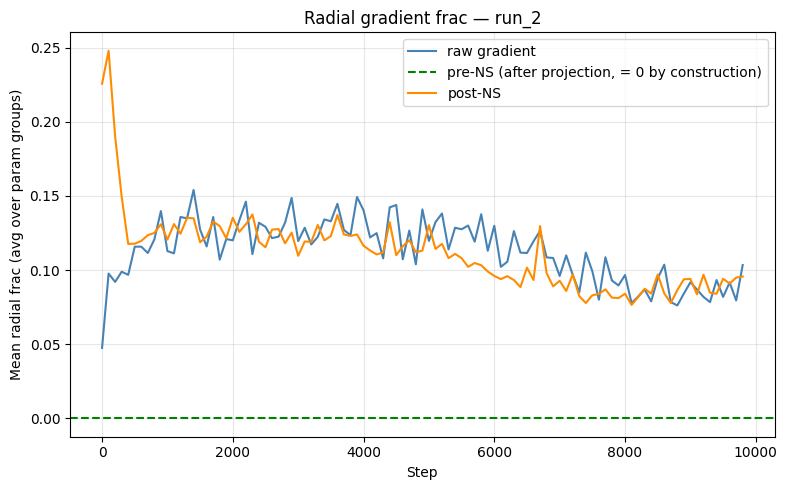
\includegraphics[width=0.8\linewidth]{radial_frac_training.png}
    \caption{Radial mass fraction plotted over training steps. Blue line represents the raw gradient's radial mass fraction, and the orange line represents the post Newton Schulz radial mass fraction. Note that this plot does not account for the direction of radial alignment, and that raw gradients are projected to 0 radial alignment prior to Newton Schulz.}
    \label{fig:placeholder}
\end{figure}

Interestingly, it seems that Newton Schulz has injected the radially aligned information (at least, an approximately equal amount of radial mass) back into our updates. How is this possible if we have already squashed all of the radial signal in our update? 

Here we offer a mechanistic explanation as to why this phenomenon occurs. We first model a gradient update $G$ with its correlation to a weight matrix $W$ under two assumptions: first, in a hypersphere constrained model, the weight matrices are approximately orthogonal \footnote{See 'Extra' section for supporting evidence}, and second, that activations are $W$ correlated from their computation, and momentum accumulates gradients that are $W$ aligned. Then, for some matrix $A$, we model $G=WA$. Now we attempt to provide some intuition as to how Newton Schulz reconstructs this radial alignment, from a mechanistic approach.

\subsection{Newton Schulz Radial Reconstruction}

We have a weight matrix $W$ whose rows are unit vectors and approximately orthogonal to each other (this is what Muon and nGPT push $W$ toward). 

The radial component of row $i$ of $G$ is the part that points along $W_i$. On nGPT, radial updates do nothing, because normalization erases them. So the natural fix is: project out the radial part of $G$ before applying NS.

The claim: this doesn't work. NS puts the radial component back. Here's why.

Let $D=\mathrm{diag}(GW^\top)$ be the diagonal matrix whose $i$-th entry is is the dot product representing the radial alignment of each row of $G$ with each row of $W$.

\[
G_\text{tan} = G - DW.
\]
This still has the form ``$W$ times something'':
\[
G_\text{tan} = WA - DW = WA - WW^\top D W = W(A - W^\top D W).
\]
The middle step uses $WW^\top = I$ our assumption that $W$ is approximately orthogonal. So $G_\text{tan} = WB$ for $B = A - W^\top D W$. The main idea here is that the left multiplication of $W$ stays, even after the projection.

Now we show that Newton Schulz preserves this structure. Take the SVD $B = P\Sigma Q^\top$. Then
\[
G_\text{tan} = WB = (WP)\,\Sigma\, Q^\top.
\]
NS replaces all singular values with 1, giving
\[
H = \mathrm{NS}(G_\text{tan}) = WPQ^\top.
\]
The key fact is that projecting out radial components doesn't break the $W\cdot(\cdot)$ structure because $G_{\text{tan}}=WB$. Newton Schulz then operates on this structured matrix. While we don't have a clean proof of why projection cannot suppress the radial mass, the empirical findings below suggest that
W-correlation in B propagates through NS and produces nonzero radial components in the output.

The general intuition for why the radial mass is so similar to the pre-projected gradient is that even after subtracting away the radial component of our update, the gradient remains highly correlated with the rows of $W$, and thus the Newton Schulz computation does not operate on an uncorrelated matrix as we hoped. Why does it recover the original alignment so accurately? This is a result that I am unable to prove. I had Claude try to come up with a rigorous proof, but it produced a long proof that I understood very little of, along with an uncertain lower bound for the radial alignment.

\\

\subsection{Experimental Results}
Now we provide empirical evidence supporting this hypothesis, as well as an interesting observation suggesting that while Newton Schulz preserves the radial mass of a pre-projected gradient, it actually inverts the direction of the radial alignment.

We run two experiments. One using randomly generated matrices $W_1, W_2$ to model a gradient matrix $G=\alpha\cdot W_1+(1-\alpha)\cdot W_2$. We vary the value of $\alpha$, project the matrix's radial component with $W_1$, and run Newton Schulz on this tangential matrix to compute the final radial alignment. Secondly, we plot the radial alignment behavior of different kinds of constructions of $G$ in order to support our theory that the preservation of left multiplication of $W$ when subtracting the radial component is what leads to the post Newton Schulz correlation.

\begin{figure}[H]
     \centering
     \begin{subfigure}[b]{0.45\textwidth}
         \centering
         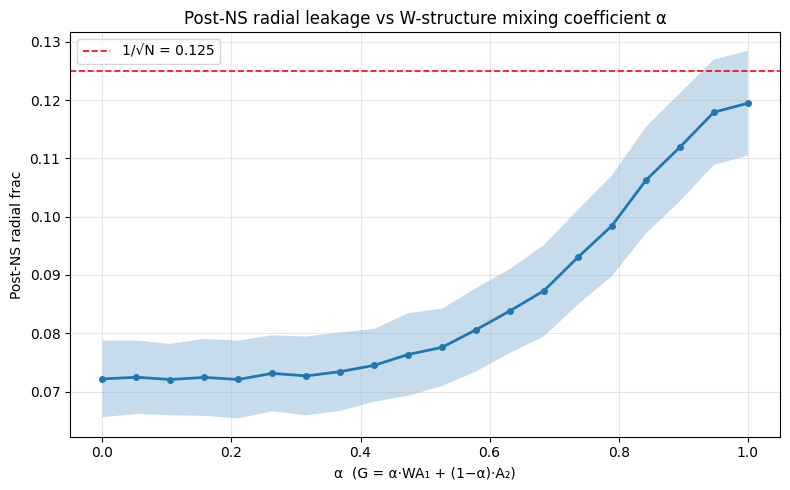
\includegraphics[width=\textwidth]{correlation_evidence.png}
         \caption{Recovered radial alignment with $W$ for matrices of the form $G=\alpha\cdot W_1 + (1-\alpha)\cdot W_2$}
         \label{fig:plot_left}
     \end{subfigure}
     \hfill
     \begin{subfigure}[b]{0.45\textwidth}
         \centering
         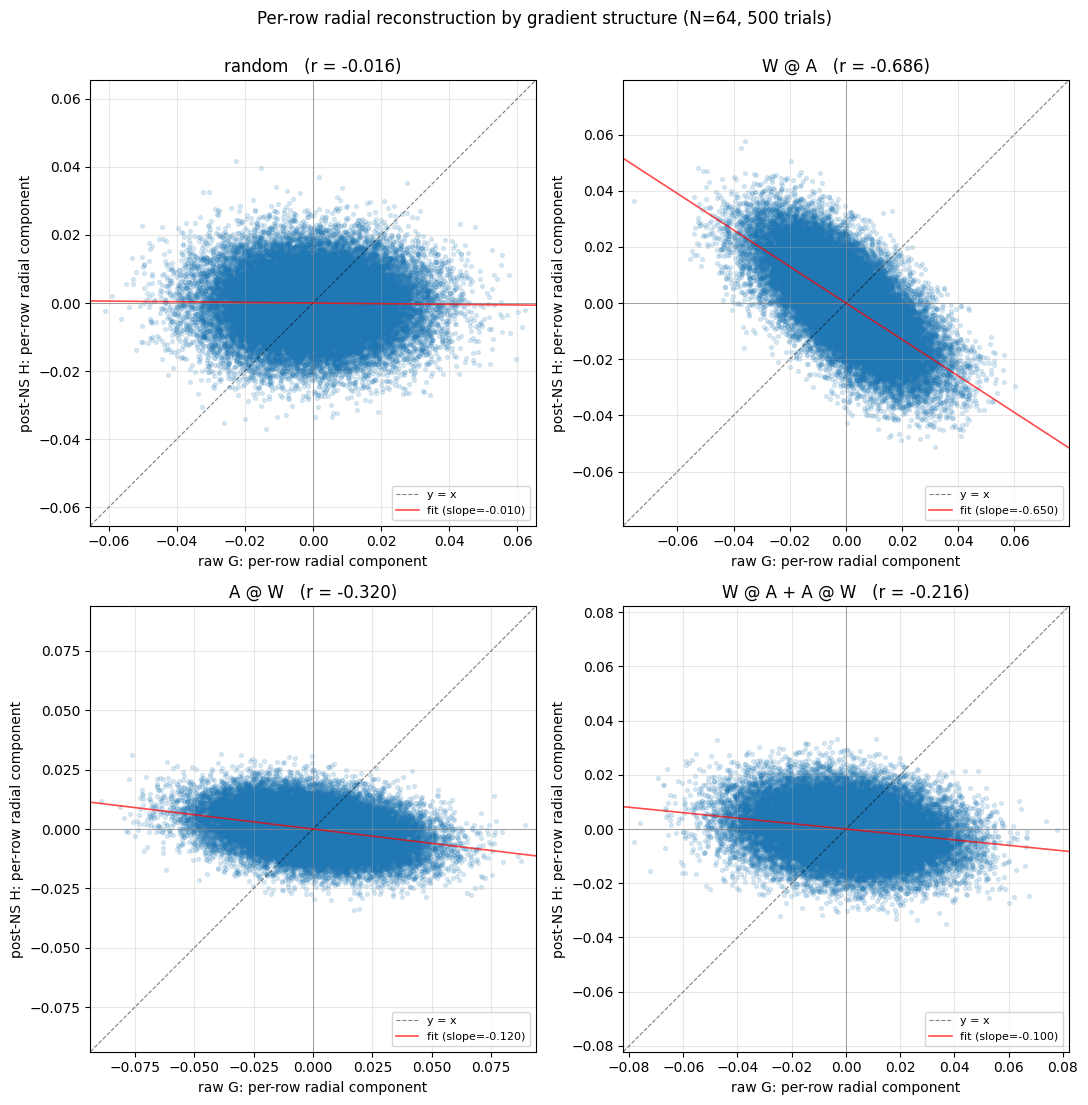
\includegraphics[width=\textwidth]{correlation.png}
         \caption{Recovered radial alignment of matrices with different constructions w.r.t $W$}
         \label{fig:plot_right}
     \end{subfigure}
     \caption{Recovered radial alignment increases with $G$'s correlation to $A$. Figure (b) indicates that the direction of the recovered radial mass is actually inverted.}
     \label{fig:total_figure}
\end{figure}

The increasing trajectory of the graph in Figure (a) provides evidence that the more correlated $G$ is with $W$, the higher the post-projection Newton Schulz alignment with $A$ will be, despite the fact we get rid of any prior radial alignment. This finding is significant and supports our assumption that gradients in our actual model are highly correlated with the weights of the model. Furthermore, in Figure (b), we find that Newton Schulz actually inverts the direction of radial alignment, which is insignificant to us since the normalization layers of the nGPT discard the information. Regardless, the behavior of Newton Schulz and the radial component is extremely interesting, and the slope of $-0.65$ supports our idea that the radial mass is recovered.

\\

More broadly, operations that don't break the $WA$ structure of the gradient will produce a similar result. Thus we propose a structural barrier to the naive adaption of Muon to the hypersphere. Newton Schulz will reliably reinject the radial information, and thus an effective change to recover the wasted effort spend on the radial signal would entail editing the Newton Schulz operation, or finding a way to decorrelated the gradient without losing meaningful information.

\section{Conclusion, Future Work, and Reflection}

In the end, we present initial findings about the behavior of Newton Schulz and the radial component of updates produced by Muon. Our intuition that $G$ is correlated with $W$ is supported by empirical evidence, but the proof of the mechanism explaining it remains an unsolved and open question.

\\

This project was a fun tangent to the original Parameter Golf challenge. Although I did not end up developing an competitive pull request, it was insightful to learn about manifold constrained architectures. Furthermore, I developed some research habits to carry forward in my future projects. Specifically, I learned how to reasonably scope experiments and produce clean sweeps to see what changes produced benefits.

\\

For my future work, I plan to continue doing projects in interpretability. I will likely not conduct any independent projects for the next five weeks as I have a final project for a compressed sensing class, and a theoretical probability class that I need to complete. I will try to tailor both of these to my machine learning interests, and if the projects end up being successful, I'll publish them on my blog post. Until then!

\section{Extra}

Here are the plots and experiments that I ran referenced in the footnotes. I will just paste the plots here, in order of the footnotes. If you are interested in any other experiments that I ran, please reach out to me.

\begin{figure}[H]
    \centering
    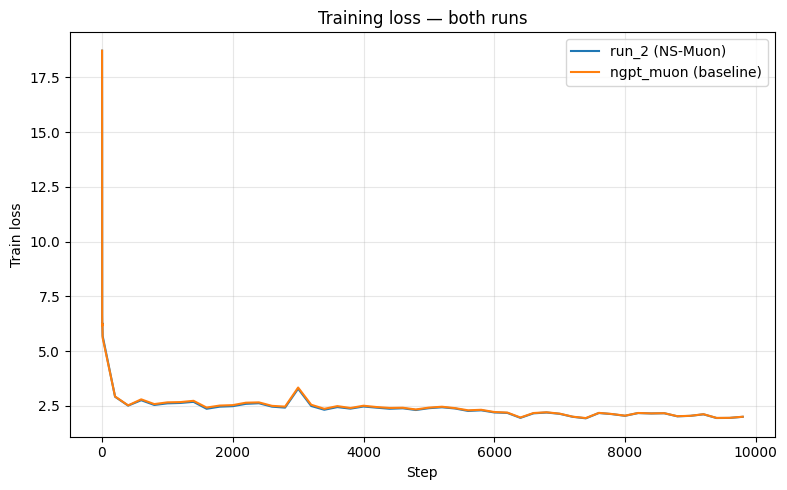
\includegraphics[width=0.8\linewidth]{output.png}
    \caption{Training loss measured over all 9810 training steps. Shows no significant improvement from the naive projection.}
    \label{fig:placeholder}
\end{figure}

\begin{figure}[H]
    \centering
    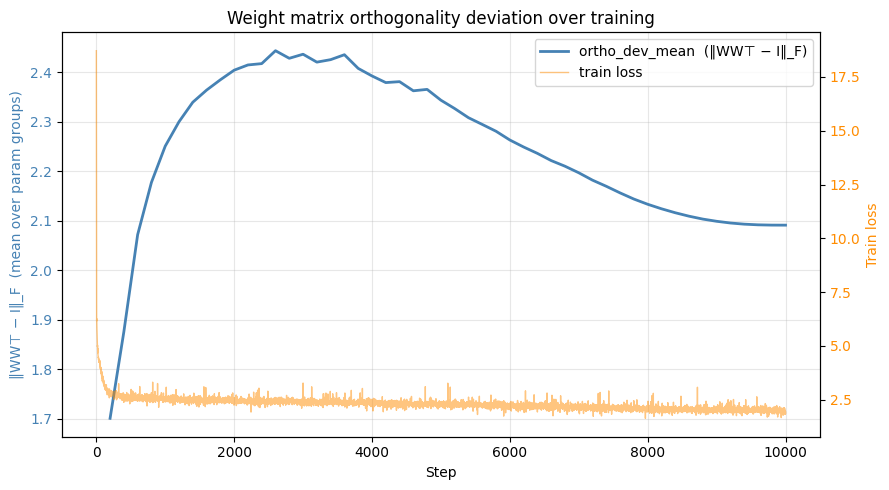
\includegraphics[width=0.8\linewidth]{orthogonality.png}
    \caption{Orthogonality of weight matrices throughout training. Random baseline is estimated to hover around $22.0$}
    \label{fig:placeholder}
\end{figure}

\end{document}
